\chapter{コンパイラのBootstrap}
\label{solv}

本章では、低遅延な広域Layer 2ネットワークを構築するにあたり想定する環境を整理した上で、本研究で
提案するシステムの概要について述べる。

\section{Bootstrapの利点}

\begin{figure}
	\begin{center}
		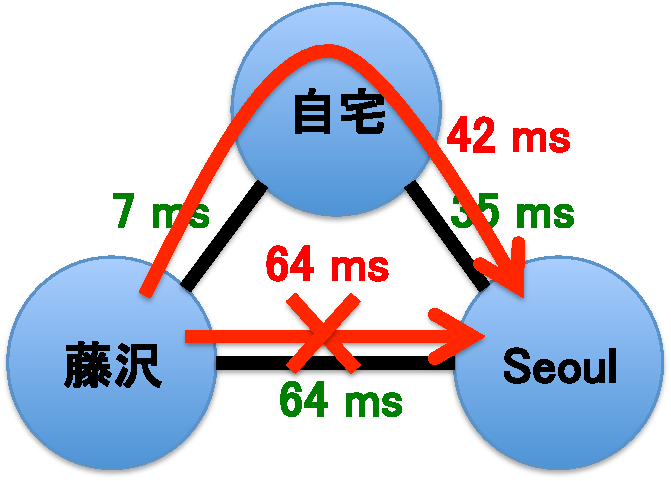
\includegraphics[scale=0.60]{./img/betterpath}
		\caption{他拠点を経由させることによる遅延の削減}
		\label{img:betterpath}
	\end{center}
\end{figure}

本研究では、まずトンネル終端点が、トンネル終端点間の遅延を計測し、その計測結果に基づいた経路選択が行えるようにする。
例えば、図~\ref{img:betterpath}で示すように、藤沢、自宅とソウルの3拠点に同一のLayer 2ネットワークを拡張するとする。この場合、
藤沢とソウルの間で通信するにあたり、インターネットの経路で直接転送するよりも、自宅を経由
することにより約35\%小さい遅延で通信することが可能である。Layer 2ネットワーク拡張技術は、このような経路を発見するために、
Layer 2ネットワークに参加している全トンネル終端点の遅延を計測する。そして、遅延が最も小さくなる経路を計測結果から計算し、その経路でイーサネットフレームの
転送を行う。

また、インターネット上で分散して動作するよう、トンネル終端点が個々でLayer 2ネットワークに参加しているトンネル終端点のリスト
を管理するようにする。トンネル終端点はLayer 2ネットワークへの参加や離脱などのメッセージを、Layer 2ネットワークに参加している
全てのトンネル終端点に広告する。これにより、全てのトンネル終端点でLayer 2ネットワークに参加しているトンネル終端点のリストを共有する。
また、全てのトンネル終端点に転送する必要があるイーサネットフレームは、SupernodeやIPマルチキャストに転送するのではなく、全てのトンネル終端点に1つ1つ転送する。
これにより、SupernodeやIPマルチキャストが不要となり、インターネット上で分散して動作するLayer 2ネットワークを構築することができる。


\section{Bootstrapの事例}
\label{solv:env}

本研究の目的は、インターネット上でサービスを提供しているサービスプロバイダーが、
インターネット上に分散された複数の拠点に同一のLayer 2ネットワークを拡張する際に、拡張されたLayer 2ネットワーク上で
動作するサービスの遅延によるパフォーマンス低下を小さくすることである。
拠点の数は数十拠点を想定する。また、拠点の場所は国内、及び、その近隣諸国とする。インターネット上
に拠点が分散しているような環境では、現在のインターネットに存在する経路の問題に
より、宛先と直接通信するより、別の拠点を経由して宛先に到達するほうが
低遅延で通信できる場合がある。そこで本研究では、遅延を小さくするために、イーサネットフレームを転送する際に
遅延の最も小さい経路で転送をすることができるLayer 2ネットワーク拡張技術を提案する。これが実現することにより、従来の手法
と比べ、拡張されたLayer 2ネットワーク上で動作するアプリケーション
のパフォーマンスが向上されることが期待される。

本研究では拡張されたLayer 2ネットワーク上で利用されるアプリケーションとしてNFSv3を
想定する。複数の拠点に分散したサービスを構築するためには、同じデータを全拠点
からアクセスできることが必要となる場合がある。複数の拠点から共通のデータを利用する手段として
NFSv3を利用するという手法が挙げられる。しかし、NFSv3は遅延がとても小さい、単一の拠点内で運用され
るように設計されているため、遅延の大きい環境で利用した場合、パフォーマンスが著しく低下する。本研究では
このような低遅延を要求するアプリケーションを想定アプリケーションとする。

\section{Bootstrapの課題}
\label{solv:requirements}

前節で説明したような環境で、低遅延な拡張されたLayer 2ネットワークを実現するための
Layer 2ネットワーク拡張技術に対する要件は以下の通りである。

\begin{itemize}
	\item{インターネット上に分散された複数の拠点へのLayer 2ネットワークの拡張}
	\item{宛先に応じた転送先の選択}
	\item{遅延の最も小さい経路でのイーサネットフレームの転送}
	\item{分散して動作すること}
\end{itemize}

低遅延な拡張されたLayer 2ネットワークを構築するためには、遅延の最も小さい経路でイーサネットフレームが転送
される必要がある。これを実現するために、まずLayer 2ネットワーク拡張技術は参加している全てのトンネル終端点間の
遅延を計測し、その計測結果を用いて遅延が最も小さい経路を計算する。そしてトンネル終端点が、
イーサネットフレームを転送する際には、イーサネットフレームの宛先に応じて転送するトンネル終端点を選択し、
計算した経路に基いて転送を行う。宛先の
トンネル終端点に直接転送する場合が最も遅延の小さい経路の場合には直接転送をする。他のトンネル終端点を経由して宛先
に転送したほうが小さい遅延で転送できる場合は、他のトンネル終端点を中継する。また、
インターネット上に分散された複数の拠点にLayer 2ネットワークを拡張することができる必要がある。
さらに、どこかの拠点で障害が発生した場合でも、正常にLayer 2ネットワークが動作していることが求められる。
そのため、Supernodeなどといった中心となるサーバーやIPマルチキャストが必要なく、分散して動作する必要がある。

%%% Local Variables:
%%% mode: japanese-latex
%%% TeX-master: "../yummy_bthesis"
%%% End:
